\subsection{GLM–HMM identifies states with varying dorsomedial striatum dependence}
\label{sec:glmhmm:2.2.8}

We examined the state-dependent weights of the GLM–HMM and found substantial differences across states in the weighting of sensory evidence, previous choice and, most intriguingly, inhibition of DMS pathways (Fig. \ref{fig:glmhmm:6}a,b). In particular, two of the three states (states 1 and 2) displayed a large weighting of sensory evidence on choice, while the ‘laser’ weight was large only in state 2. In contrast, in state 3, choice history had a larger weight than in the other states, and neither sensory evidence nor ‘laser’ had much influence on choice.

To characterize state-dependent psychometric performance, we used the fitted model to compute the posterior probability of each state given the choice data and assigned each trial to its most probable state (Fig. \ref{fig:glmhmm:6}c,d). We then examined the psychometric curves for trials assigned to each state. In state 3, performance was low (Fig. \ref{fig:glmhmm:6}g) and DMS inhibition had little effect on behavior (Fig. \ref{fig:glmhmm:6}c,d). This is consistent with the high GLM weight on choice history in this state and low weights on sensory evidence and laser (Fig. \ref{fig:glmhmm:6}a,b). This implies relatively little contribution of DMS pathways during a task-disengaged state when mice pursued a strategy of repeating previous choices rather than accumulating sensory evidence. When considered together with comparisons of the effect of pathway-specific DMS inhibition in control T-maze tasks where performance is high (Fig. \ref{fig:glmhmm:2}c) but effects of inhibition are limited (Fig. \ref{fig:glmhmm:3}f–k and Extended Data Fig. \ref{fig:ap1:ext5}b,c), this implies a dissociation between task performance and the contributions of DMS pathways to behavior.

\begin{figure}[t!]
  \begin{center}
    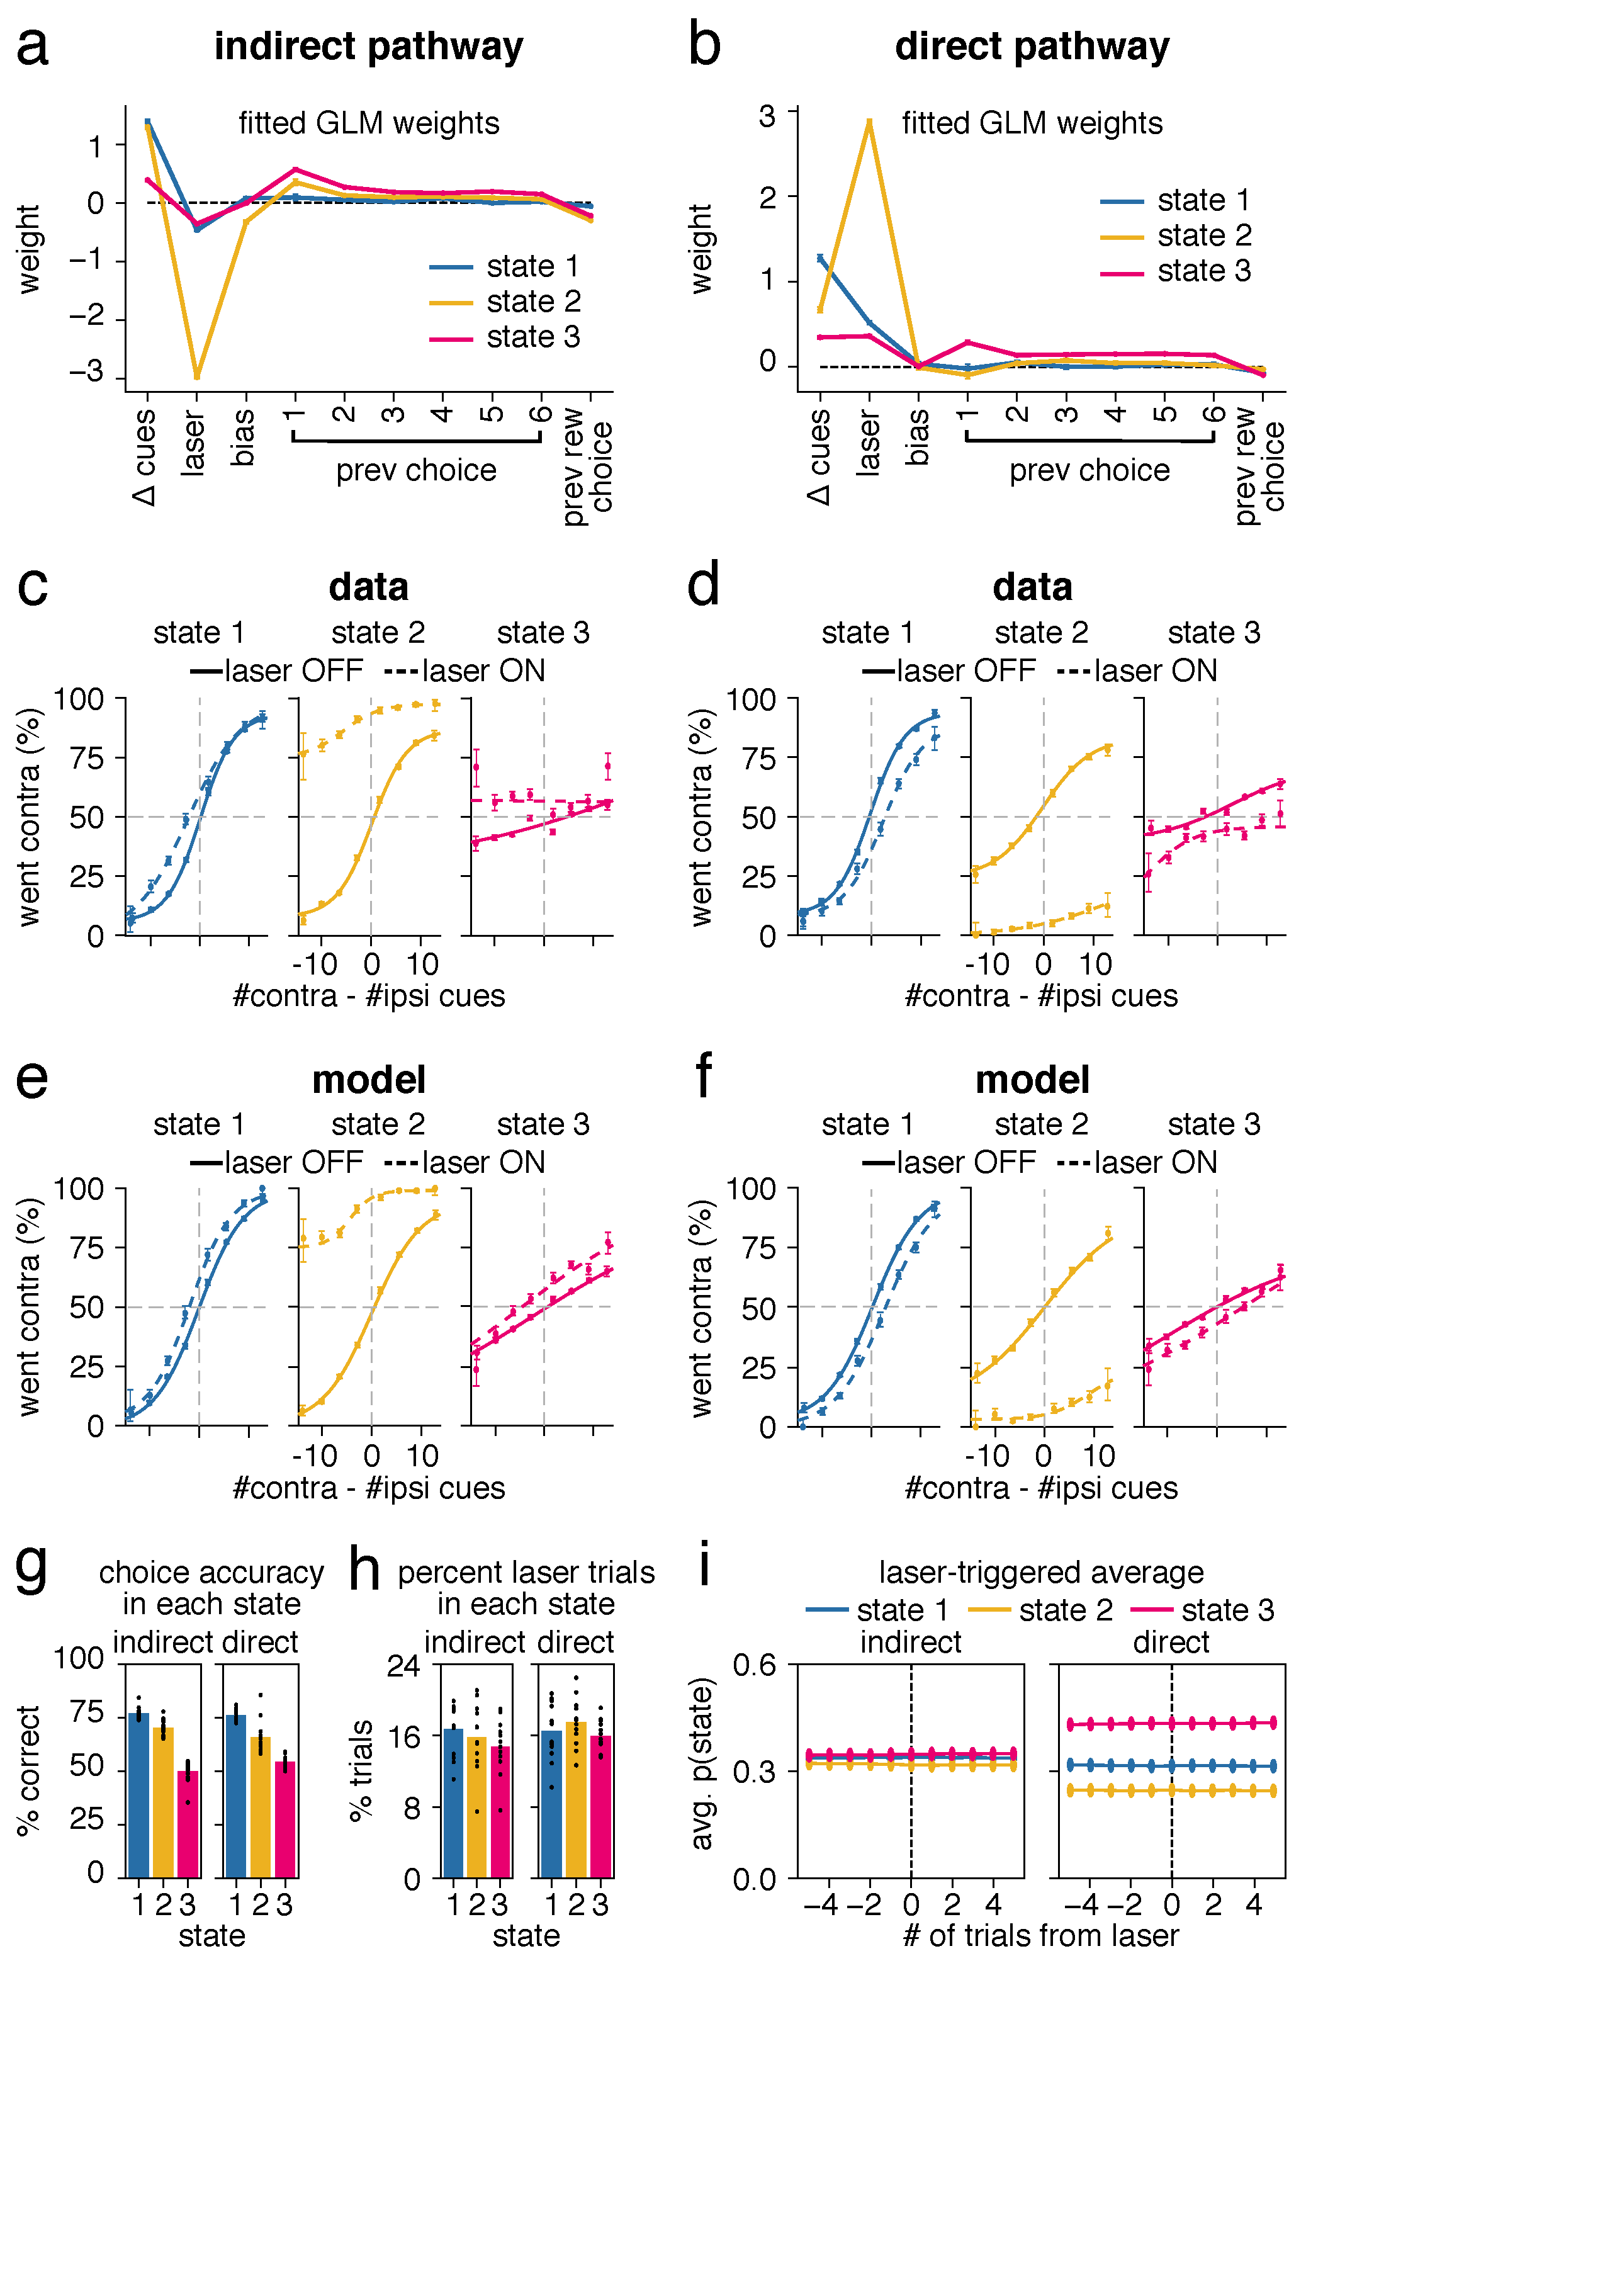
\includegraphics[width=0.80\linewidth]{ch2-glmhmm/glmhmm-figures/Fig6.pdf}
    \caption[A GLM–HMM uncovers states during the evidence accumulation task with different weighting on sensory evidence, choice history and dorsomedial striatum pathway inhibition]{\textbf{A GLM–HMM uncovers states during the evidence accumulation task with different weighting on sensory evidence, choice history and dorsomedial striatum pathway inhibition.} (a) Fitted GLM weights for 3-state model from mice in the indirect pathway DMS inhibition group. Error bars denote ($\pm$1) posterior standard deviation for each weight. The magnitude of the weight represents the relative importance of that covariate in predicting choice, whereas the sign of the weight indicates the side bias (e.g. a negative laser weight indicates that if inhibition}
    \label{fig:glmhmm:6}
  \end{center}
  \vspace{-1.5cm}
\end{figure}
\begin{figure}[t!]
  \contcaption{is in the right hemisphere, the mice will be more likely to turn left, while a positive weight on previous choice indicates that if the previous choice was to the right, in the current trial this will bias the mice to turn right again). (b) Same as a but for the direct pathway group. (c) Fraction of contralateral choices as a function of the difference in contralateral versus ipsilateral cues in each trial for mice in the indirect pathway inhibition group. To compute psychometric functions, trials were assigned to each state by taking the maximum of the model’s posterior state probabilities on each trial. Error bars denote $\pm$1 SEM  for light off (solid) and light on (dotted) trials. Solid curves denote logistic fits to the concatenated data across mice for light off (solid) and light on (dotted) trials.  (d) Same as c but for the mice receiving direct pathway inhibition of the DMS. (e) Same as c but for data simulated from the model fit to mice receiving indirect pathway inhibition of the DMS  (see \ref{sec:appendix1:methods}). (f). Same as e but for mice receiving direct pathway inhibition of the DMS. (g) Performance in each state for mice receiving DMS inhibition in the indirect pathway (left) and direct pathway (right), shown as the percentage of total trials assigned to that state in which the mice made the correct choice. Colored bars denote the average performance across all mice. Black dots show averages for individual mice (n=13 mice for both groups). (h) Percentage of laser-on trials that the model assigned to each state for mice receiving DMS inhibition in the indirect pathway (left) and direct pathway (right). Colored bars denote the average performance across all mice. Black dots show averages for individual mice (n=13 mice for both groups). (I) The posterior probability of each state for the five trials before and after a laser-on trial, averaged across all such periods (n=8570, indirect; n=7927, direct). }% Continued caption
\end{figure}

Compared to state 3, sensory evidence heavily modulated behavior in both states 1 and 2, and performance was accordingly high (Fig. \ref{fig:glmhmm:6}c,d,g). Interestingly, the effect of DMS pathway inhibition was much larger in state 2. These results were again consistent with the GLM weights: both state 1 and 2 had high weighting of sensory evidence and low weighting of choice history but greatly differed in their weighting of the ‘laser’ (Fig. \ref{fig:glmhmm:6}a,b). The discovery of state 2 implies that DMS pathways contribute most heavily to choices in a state in which mice are pursuing a strategy of evidence accumulation, consistent with cross-task comparisons of the effects of inhibition (Fig. \ref{fig:glmhmm:3}). The discovery of state 1, which differed most noticeably from state 2 in the extent that the laser affected choice, may suggest the existence of another neural mechanism for evidence accumulation with minimal DMS dependence.

We found that GLM–HMM simulations closely recapitulated these state-dependent psychometric curves (Fig. \ref{fig:glmhmm:6}e,f). This not only validated our fitting procedure but provided additional evidence that a multistate model provides a good account of the animals’ decision-making behavior during the evidence accumulation task.

While the effect of the laser differed across states, the probability of being in a particular state did not change on or after trials with optical inhibition (Fig. \ref{fig:glmhmm:6}i), implying that DMS pathway inhibition itself did not generate transitions between states. In addition, the fraction of trials with optical inhibition was equivalent across states ($\sim$15\% of all trials in each state; Fig. \ref{fig:glmhmm:6}h). This implies that the model did not identify states simply based on the presence of laser trials.

We obtained similar states when fitting the model to a combined dataset including all groups of mice (those receiving DMS indirect and direct pathway inhibition, as well as control mice receiving DMS illumination in the absence of NpHR; Extended Data Fig. \ref{fig:ap1:ext7}f). As when fitting each group separately, the combined fit revealed that both inhibition groups contained a single state with large weights on sensory evidence and the laser. In contrast, the control mice had small laser weights across all three states.

We also examined the results of fitting the four-state GLM–HMM (Extended Data Fig. \ref{fig:ap1:ext7}d,e), given it had a slightly higher cross-validated log-likelihood than the three-state model (Extended Data Fig. \ref{fig:ap1:ext7}a). In this case, the weights for states 1 and 2 were very similar to those in the three-state model; the key difference was that the choice history state (state 3 of the three-state model) was further subdivided into two states that differed in having a slight rightward versus a slight leftward bias. This suggests that while the model may uncover finer-grained structure in the data beyond three states (Extended Data Fig. \ref{fig:ap1:ext7}d,e), these states yield diminishing interpretive insight on the weighting of sensory evidence, choice history and DMS pathway inhibition across time.